\section{Pixelar}
\par{Este filtro consiste en tomar bloques de 2x2 píxeles y asignarles a estos el promedio del bloque. De esta manera se disminuye la calidad de la imagen.}
\subsection{Código C}
\par{El código de C consiste en recorrer la imagen de a dos filas y dos columnas por iteración. En cada iteración se calcula el promedio de los canales de los píxeles.}
\par{A continuación adjuntamos el pseudocódigo.}

\begin{algorithm}[h!]
\caption{Promedio}
\begin{algorithmic}
  \Function{promedio}{$a :~unsigned~ char, ~b:~ unsigned ~char, ~c: ~unsigned~ char, ~d: ~unsigned~ char$}  $\to \texttt{float}$
	\State $float~ af \gets a$
	\State $float~ bf \gets b$
	\State $float~ cf \gets c$
	\State $float~ df \gets d$
	\State \Return $(af/4+bf/4+cf/4+df/4)$
	
\EndFunction
\end{algorithmic} 
\end{algorithm}	
	
	\begin{algorithm}[h!]
\caption{Pixelar}
\begin{algorithmic}
  \Function{pixelar}{src: *unsigned char, dst: *unsigned char, cols: int, filas: int, srcRowSize: int, dstRowSize: int}
	\State $unsigned~ char~ (*srcMatrix)[srcRowSize] = (unsigned~ char (*)[srcRowSize])~ src$
	\State $unsigned~ char~ (*dstMatrix)[dstRowSize] = (unsigned~ char (*)[dstRowSize])~ dst$
	
	\For{$f \gets 0~..~filas-1; f+=2$}
		\For{$c \gets 0~..~cols-1; c+=2$}
			\State $bgra_t* p_s1 \gets (bgra_t*)$ \& $srcMatrix[f][c * 4]$
			\State $bgra_t *p_d1 \gets (bgra_t*)$ \&$dstMatrix[f][c * 4]$
			
			\State $bgra_t* p_s2 \gets (bgra_t*)$ \& $srcMatrix[f+1][c * 4]$
			\State $bgra_t *p_d2 \gets (bgra_t*)$ \&$dstMatrix[f+1][c * 4]$
			
			\State $bgra_t* p_s3 \gets (bgra_t*)$ \& $srcMatrix[f+1][(c+1) * 4]$
			\State $bgra_t *p_d3 \gets (bgra_t*)$ \&$dstMatrix[f+1][(c+1) * 4]$
			
			\State $bgra_t* p_s4 \gets (bgra_t*)$ \& $srcMatrix[f][(c+1) * 4]$
			\State $bgra_t *p_d4 \gets (bgra_t*)$ \&$dstMatrix[f][(c+1) * 4]$
			
			\State k $\gets$ 0.5
			
			\State b $\gets$ \Call{promedio}{$p_s \rightarrow b, p_s2 \rightarrow b, p_s3 \rightarrow b, p_s4 \rightarrow b$}
			\State g $\gets$ \Call{promedio}{$p_s \rightarrow g, p_s2 \rightarrow g,p_s3 \rightarrow g, p_s4 \rightarrow g$}
			\State r $\gets$ \Call{promedio}{$p_s \rightarrow r, p_s2 \rightarrow r, p_s3 \rightarrow r, p_s4 \rightarrow r$}
			\State a $\gets$ \Call{promedio}{$p_s \rightarrow a, p_s2 \rightarrow a, p_s3 \rightarrow a, p_s4 \rightarrow a$}
				
			\For{$i \gets 1~..~4$}
				\State ($p_di \rightarrow$b) $\gets$ b
				\State ($p_di \rightarrow$g) $\gets$ g
				\State ($p_di \rightarrow$r) $\gets$ r
				\State ($p_di \rightarrow$ a) $\gets$ a
			\EndFor
		\EndFor
	\EndFor
\EndFunction

\end{algorithmic} 
\end{algorithm}
\subsection{Código ASM}
\par{El código en ASM consiste en una unión de ciclos, uno exterior para iterar sobre las filas y otro interior para iterar sobre los elementos de la misma (columnas). Lo que hace este código es en cada iteración, lee de memoria dos veces, empezando en la misma columna pero de dos filas diferentes. De esta forma levanta como una matriz de 8 elementos (4x2). Lo que se puede obtener de esta información va a servir para sobreescribir 8 píxeles.}
\par{El ciclo luego procede en extender los signos de cada byte, luego guardar la sumatoria de los elementos {1,2,6,7} (mirándolo como una matriz de 4x2), y la sumatoria de {4,5,8,9} en dos registros aparte, calcular el promedio de esto, o sea dividirlos por cuatro. Y luego a esta información la volvemos a agrupar juntas en un mismo registro que se veria de esta manera:}

\par{\textbf{XMM:}}
\xmmb{$Pp1_a$}{$Pp1_r$}{$Pp1_g$}{$Pp1_b$}{$Pp1_a$}{$Pp1_r$}{$Pp1_g$}{$Pp1_b$}{$Pp2_a$}{$Pp2_r$}{$Pp2_g$}{$Pp2_b$}{$Pp2_a$}{$Pp2_r$}{$Pp2_e$}{$Pp2_b$}
\par {Pp1 : promedio píxeles {1,2,6,7}.}
\par{Pp2 : promedio píxeles {4,5,8,9}}
	
\par{Finalmente a este registro lo escribimos en la imagen destino, en los lugares de los píxeles que levantamos en la imagen src.}
\par{Por último movemos los current en columnas 4 píxeles que es la cantidad sobre esa fila q procesamos en cada iteración. Y si terminamos de procesar la fila, nos movemos dos filas, ya que vamos procesando dos juntas a la vez.}
	
\subsection{Experimentación 1}

\subsubsection{Idea}	
\par{Comparamos la eficiencia del código en ASM, \textcolor{red}{el de C y el de C optimizado}.}
	
\subsubsection{Resultados}
	\begin{figure}[H]
	\centering
	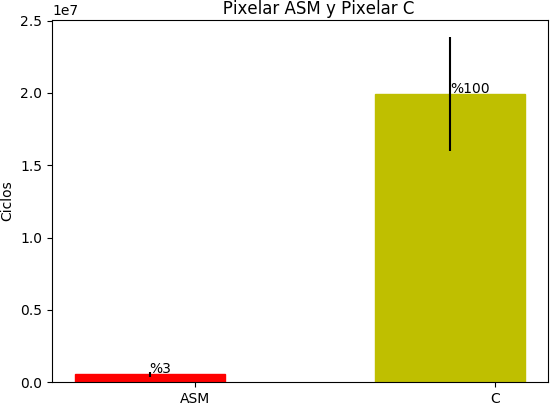
\includegraphics[width = 10 cm, height = 6.5 cm]{imagenes/ASMvsCPixelar.png}
	\caption[center]{Comparación \textcolor{red}{$\dfrac{\text{ciclos totales}}{\text{cant. de píxeles}}$} - diferentes implementaciones de C y ASM}
\end{figure}

\begin{figure}[H]
	\centering
	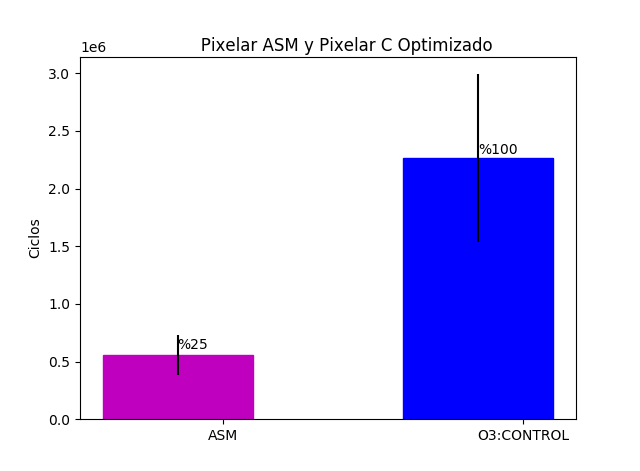
\includegraphics[width = 10 cm, height = 6.5 cm]{imagenes/PixelarvsCONTROL.png}
	\caption[center]{Comparación \textcolor{red}{$\dfrac{\text{ciclos totales}}{\text{cant. de píxeles}}$} - diferentes implementaciones de C y ASM}
\end{figure}

\subsection{Experimentación 2}
\subsubsection{Idea}
\par{Comparamos la eficiencia entre un código que utiliza instrucciones como shift, para dividir los píxeles, contra otro que usa las instrucciones para dividir floats, que implican además tener que hacer un traspaso de formato.}

\subsubsection{Hipótesis}
\par{Nuestra idea es que va a ser mucho más eficiente el código donde utilizamos las intrucciones de shift para dividir los números porque son operaciones básicas que se encarga el registro de hacerlas, en cambio \textcolor{red}{el pasar a float, dividir luego y volver a pasar a float}, son todas operaciones sin implementación primitiva (por esto nos referimos a que están compuestas de varias otras instrucciones) y esto da lugar a que la ejecución de cada una demore varios ciclos más que un simple shift.}

\subsubsection{Resultados}
\begin{figure}[H]
	\centering
	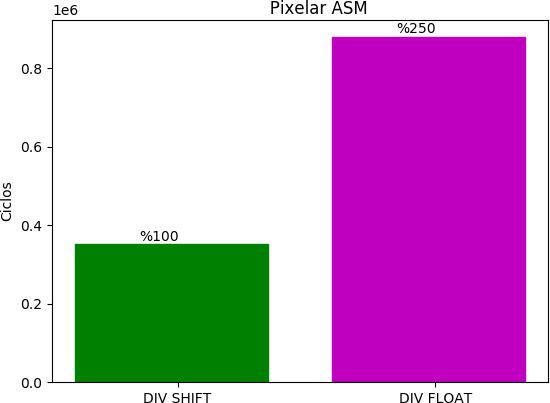
\includegraphics[width = 10 cm, height = 6 cm]{imagenes/Div_pixelar.png}
	\caption[center]{}
\end{figure}
	
\subsubsection{Conclusión}
\par{Definitivamente el código en el cual dividimos con shifts fue mucho más eficiente por lo ya explicado en la hipótesis.}